\documentclass[]{beamer}
% Class options include: notes, notesonly, handout, trans,
%                        hidesubsections, shadesubsections,
%                        inrow, blue, red, grey, brown

% Theme for beamer presentation.
\usepackage{beamerthemesplit} 
%\usepackage{moreverb}
\usepackage{listings, algorithmic}
\usepackage[normal]{subfigure}

\let\oldhat\hat
\renewcommand{\vec}[1]{\mathbf{#1}}
\renewcommand{\hat}[1]{\oldhat{\mathbf{#1}}}
% Other themes include: beamerthemebars, beamerthemelined, 
%                       beamerthemetree, beamerthemetreebars  

\title{Multi-Dimensional Aggregation for Temporal Data}    % Enter your title between curly braces
\author{Laura Bledaite\\ Supervisor: Prof. Johann Gamper}                 % Enter your name between curly braces

\institute{Free University of Bozen - Bolzano}      % Enter your institute name between curly braces
\date{\today}                    % Enter the date or \today between curly braces

\begin{document}

% Creates title page of slide show using above information
\begin{frame}
  \titlepage
\end{frame}


\section[Outline]{}

% Creates table of contents slide incorporating
% all \section and \subsection commands
\begin{frame}
  \frametitle{Outline}
  \tableofcontents
\end{frame}


\section{TMDA-CI algorithm}

\begin{frame}
 
\frametitle{TMDA-CI algorithm}   % Insert frame title between curly braces

\textbf{Idea:} Scans the argument relation (ordered by the interval start values of the tuples), produces the result tuples, and removes the old tuples from main memory.\\

\textbf{Uses: } AVL-trees for keeping the open tuples.
\end{frame}


\section{TMDA-FI algorithm}
\begin{frame}
  \frametitle{TMDA-FI algorithm}   % Insert frame title between curly braces

\begin{algorithmic}
\STATE Initialize $gt$ to $\vec{g}$ and extend it with columns $f_{A_{i_1}} , \dots , f_{A_{i_p}}$ initialized to NULL;
\STATE Create index for $gt$ on attributes $T, A_1,\dots,A_m$ ;
\FORALL{tuple $r \in \vec{r}$} 
\FORALL{$i \in LOOKUP(gt,r,θ)$}
\STATE $r^{'} \leftarrow ADJUST(r, gt[i].T, C)$; 
\FORALL{$f_j \in \vec{F}$}
\STATE $gt[i].f_{A_{i_j}} \leftarrow gt[i].f_{A_{i_j}} \bigoplus r^{'}.A_{i_1}$; 
\ENDFOR
\ENDFOR
\ENDFOR
\RETURN $gt$;
\end{algorithmic}

\end{frame}

\section{Experiments}

\subsection{Data Used}
\begin{frame}
  \frametitle{Data Used}   % Insert frame title between curly braces
  \begin{itemize}
  \item
  $r^{equal}$: $af \in [0.000001, 0.000005]$.
  \item
  $r^{seq}$: $af=1$.
  \item
  $r^{random}$: $af \in [0.023857, 0.11649]$.
  \item
  $r^{worst}$: $af \in [1.999995, 1.999999]$.
  \end{itemize}
\end{frame}


\begin{frame}
  \frametitle{Random Data}   % Insert frame title between curly braces

  \begin{figure}[ht!]
\centering 
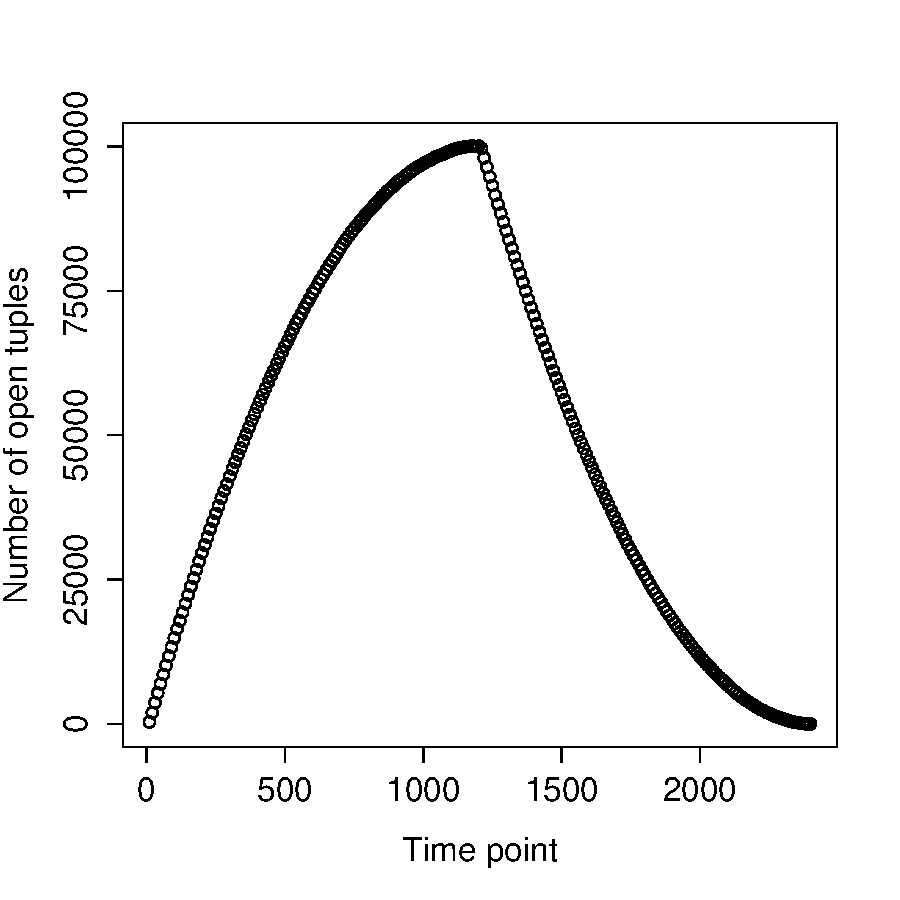
\includegraphics[width=50mm]{../graphs/random_open_tuples.pdf}
\caption{Number of open tuples in the random data set.}
\label{open_tuples} 
\end{figure}


\end{frame}

\subsection{Scalability of TMDA-CI and TMDA-FI}

\begin{frame}
  \frametitle{Scalability of TMDA-CI and TMDA-FI}   % Insert frame title between curly braces

  \begin{figure}[ht!]
	\begin{center}
		\subfigure[constant intervals]{\label{constant_tmda_ci}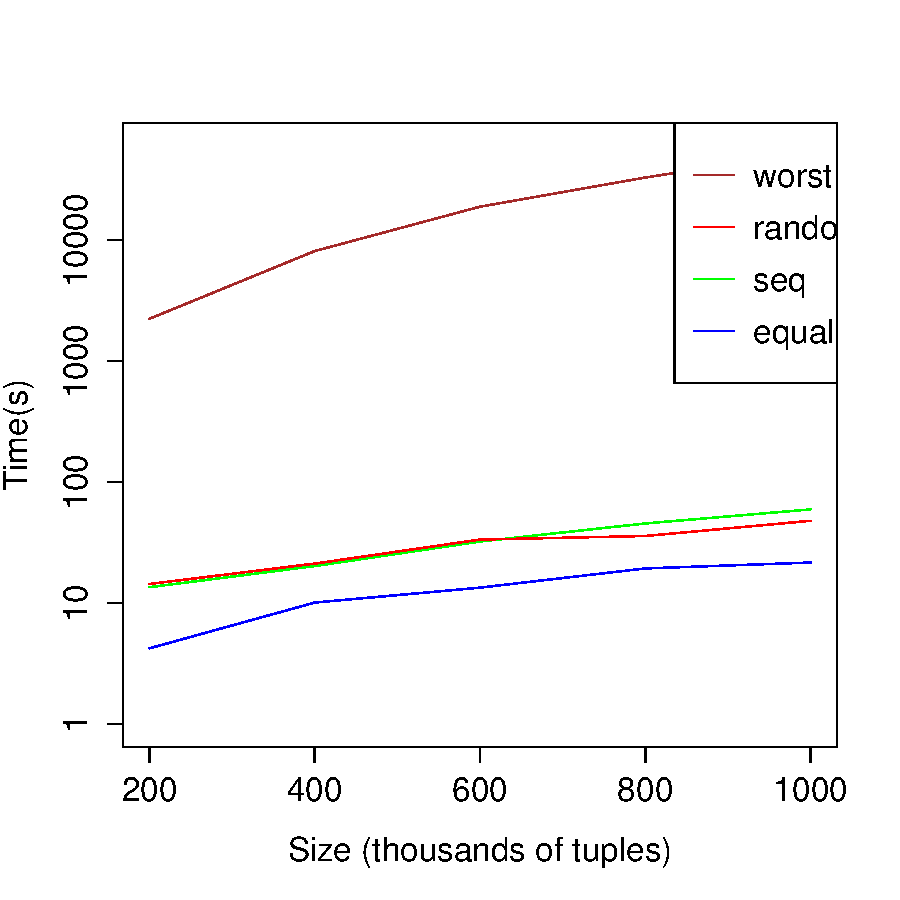
\includegraphics[width=0.4\textwidth]{../graphs/constant_tmda_ci.pdf}}
		\subfigure[fixed intervals]{\label{constant_tmda_fi}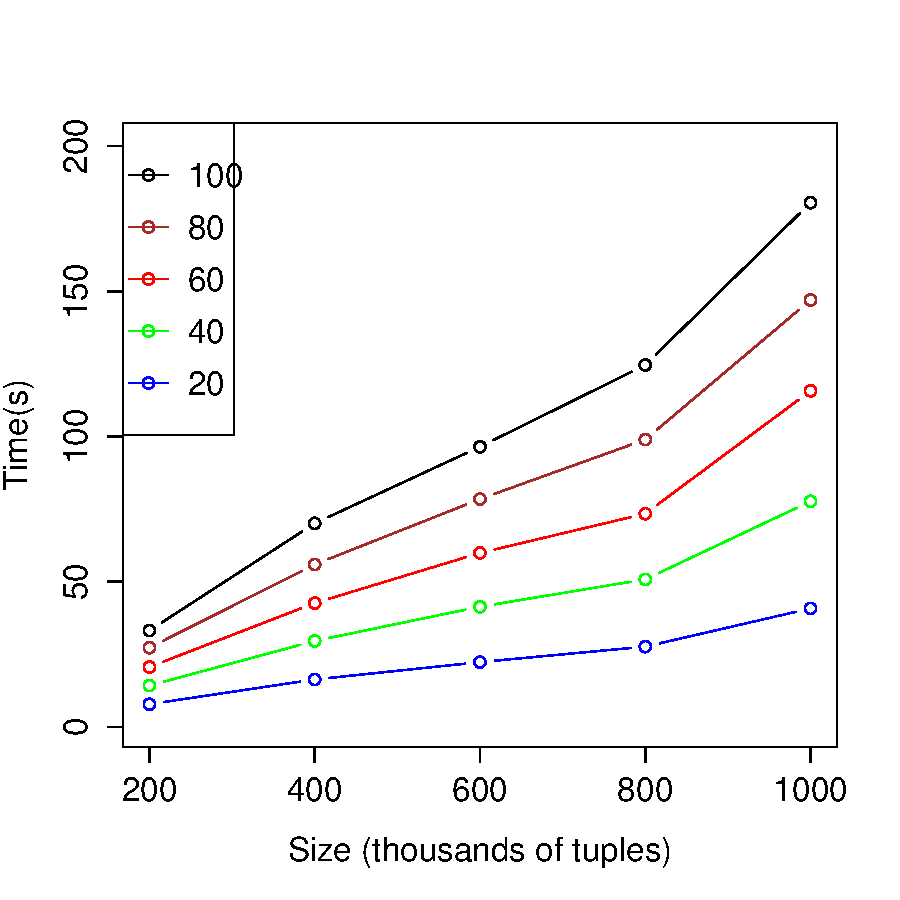
\includegraphics[width=0.4\textwidth]{../graphs/tmda_fi_scalability.pdf}}
	\end{center}
	\caption{Evaluation of TMDA-CI and TMDA-FI.}
	\label{scalability}
  \end{figure} 
\end{frame}

\subsection{Mallable vs Constant Interval Semantics}
\begin{frame}
\frametitle{Mallable vs Constant}
\begin{figure}[ht!]
	\begin{center}
		\subfigure[equal]{\label{mal_vs_const_equal}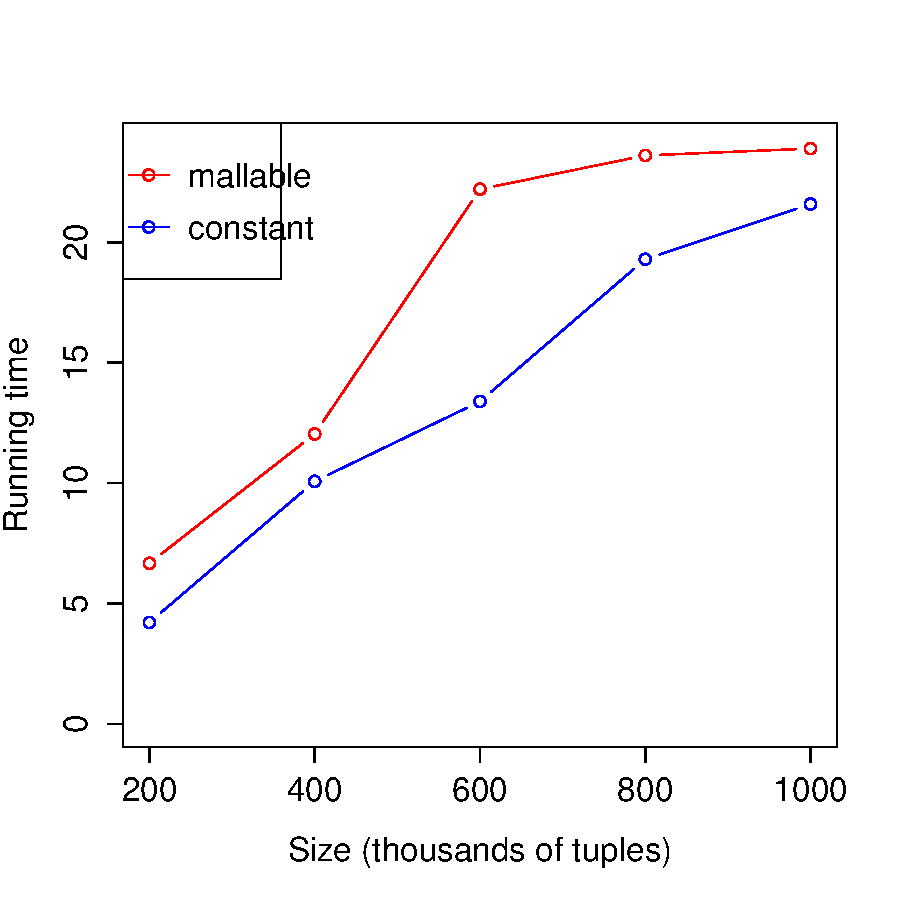
\includegraphics[width=0.3\textwidth]{../graphs/mal_vs_const_equal.pdf}}
		\subfigure[sequential]{\label{mal_vs_const_seq}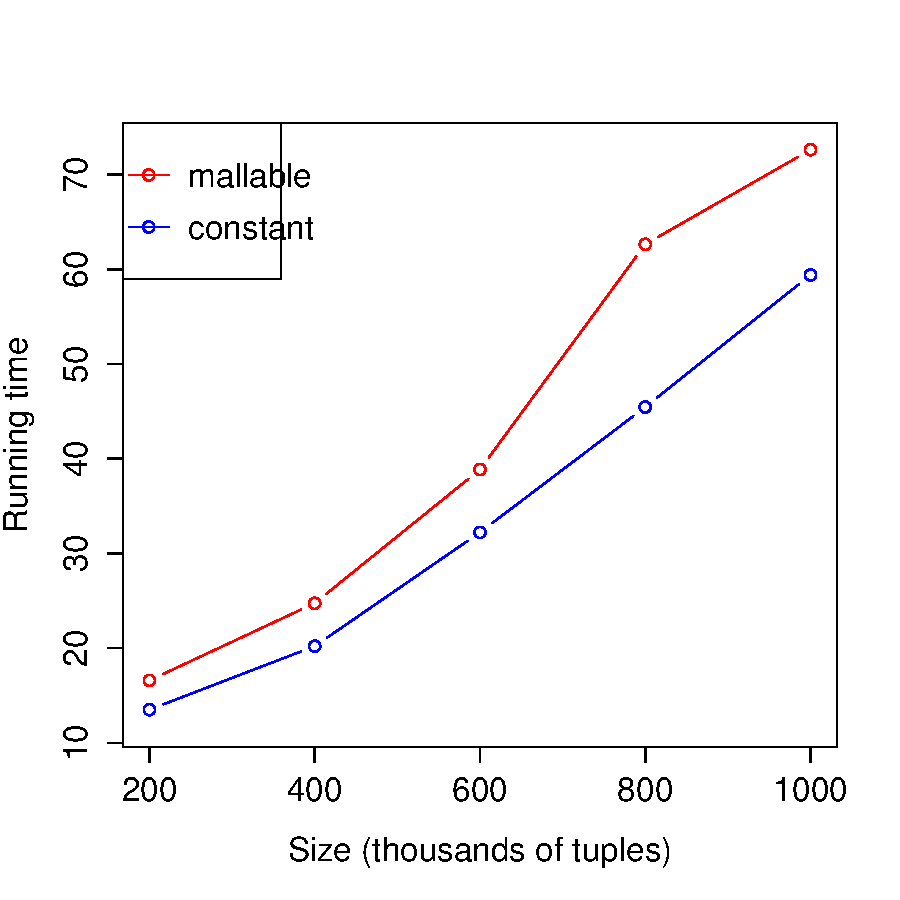
\includegraphics[width=0.3\textwidth]{../graphs/mal_vs_const_seq.pdf}}
		\subfigure[random]{\label{mal_vs_const_random}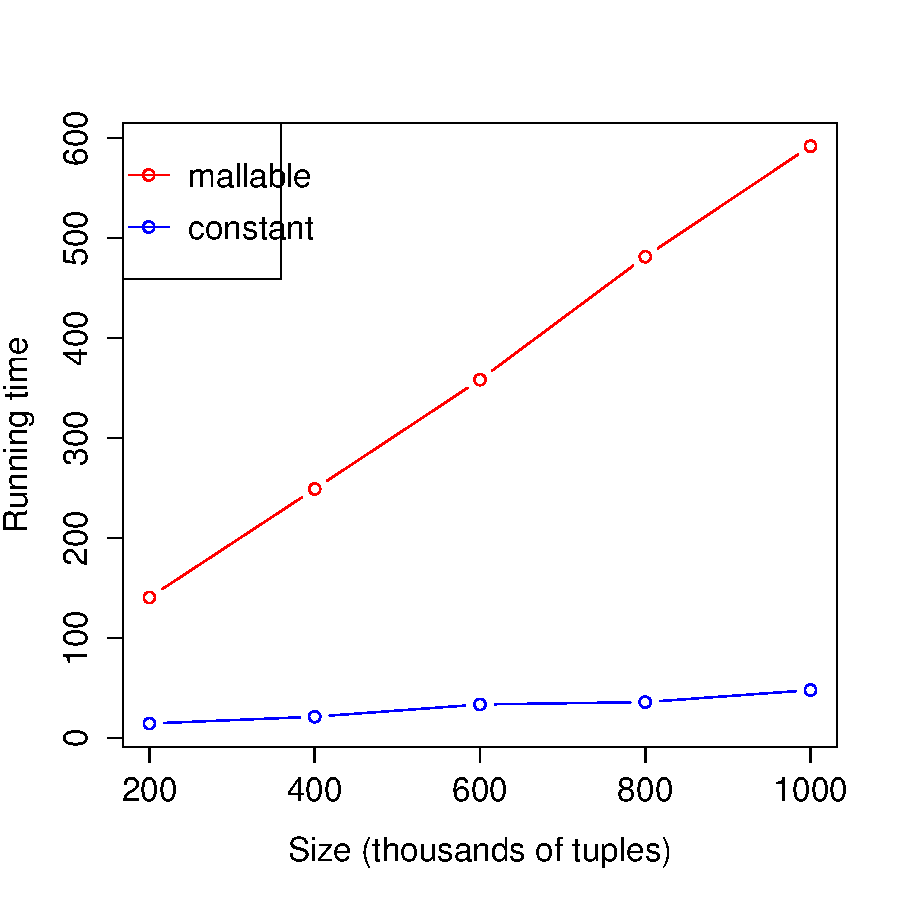
\includegraphics[width=0.3\textwidth]{../graphs/mal_vs_const_random.pdf}}
	\end{center}
	\caption{Comparison of TMDA-CI runtime with mallable and constant attribute characteristics.}
	\label{mal_vs_const}
\end{figure} 
\end{frame}

\subsection{TMDA-CI vs SQL+TMDA-FI}

\begin{frame}
\frametitle{TMDA-CI vs SQL + TMDA-FI}
\begin{figure}[ht!]
\centering 
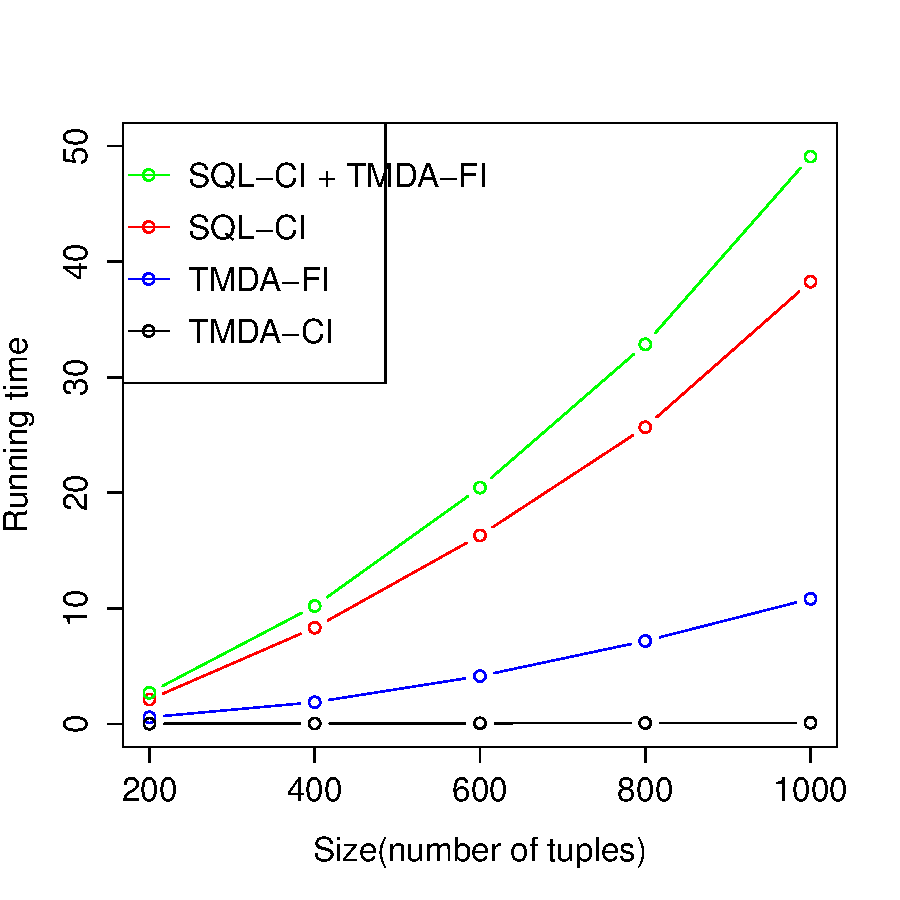
\includegraphics[width=50mm]{../graphs/sql_tmda_fi.pdf}
\caption{Constant vs Fixed Interval Semantics.}
\label{sql_tmda_fi} 
\end{figure}
\end{frame}

\section{Conclusions}
\begin{frame}
\frametitle{Conclusions}
\begin{itemize}
\item 
$r^{worst}$ is clearly "worst" for TMDA-CI;
\item
Number of groups impacts the performance of TMDA-FI;
\item
Mallable attributes add additional computation, especially for $r^{random}$;
\item
TMDA-CI is faster than SQL + TMDA-FI;
\item
Optimizations are useful.
\end{itemize}
\end{frame}

\end{document}
